\chapter{Cadre général du projet}
\label{chap:cadre-projet}

\section*{Introduction}

Ce chapitre présente le cadre général de notre projet de fin d'études. Il débute par la présentation de l'organisme d'accueil et de son environnement professionnel. Il expose ensuite le contexte du projet \textit{EcoRewind}, l'étude de l'existant, la problématique identifiée et la solution proposée. Enfin, il décrit le formalisme de modélisation et la méthodologie de travail adoptés pour la conception et la réalisation de la solution.

\section{Contexte général}

Ce stage de fin d'études s'inscrit dans le cadre de l'obtention du diplôme national d'ingénieur en informatique, spécialité Génie Logiciel, à TEK-UP. Il a été réalisé au sein d'\textbf{ASSURANCES MAGHREBIA} sur une période de six mois. La transformation numérique constitue aujourd'hui un levier essentiel pour les entreprises qui souhaitent moderniser leurs services et développer des solutions innovantes. C'est dans cette dynamique que s'inscrit notre projet, qui vise à concevoir \textit{EcoRewind}, une plateforme numérique de sensibilisation et d'accompagnement au tri sélectif des déchets en Tunisie.

\section{Organisme d'accueil}

\textbf{ASSURANCES MAGHREBIA} est une compagnie tunisienne spécialisée dans les activités d'assurance et de réassurance. Fondée en 1973, elle figure parmi les acteurs établis du secteur assurantiel tunisien et propose une offre de produits et de services destinée aux particuliers ainsi qu'aux entreprises. Son siège social est situé au \textbf{64, rue de Palestine, 1002 Tunis}. À travers son réseau de distribution et ses équipes aux compétences complémentaires, l'entreprise assure une proximité avec ses assurés et ses partenaires. ASSURANCES MAGHREBIA inscrit son développement dans une démarche d'amélioration continue, fondée sur la qualité de service, l'innovation et la modernisation de ses processus. Elle accorde ainsi une attention particulière à l'intégration des technologies numériques afin de simplifier les parcours utilisateurs, d'optimiser les opérations internes et de répondre efficacement aux attentes de ses clients. Cet environnement professionnel constitue un cadre favorable au développement de solutions innovantes et à l'acquisition de compétences pratiques dans les domaines des systèmes d'information et de la transformation digitale.

\begin{figure}[H]
    \centering
    \IfFileExists{img/maghrebia_logo.png}{%
        \includegraphics[width=0.35\textwidth]{img/maghrebia_logo.png}%
    }{%
        \fbox{\parbox[c][3cm][c]{0.35\textwidth}{\centering Logo d'ASSURANCES MAGHREBIA}}%
    }
    \caption{Logo d'ASSURANCES MAGHREBIA}
    \label{fig:maghrebia-logo}
\end{figure}

\begin{figure}[H]
    \centering
    \IfFileExists{img/maghrebia_siege.png}{%
        \includegraphics[width=0.55\textwidth]{img/maghrebia_siege.png}%
    }{%
        \fbox{\parbox[c][3cm][c]{0.55\textwidth}{\centering Siège social d'ASSURANCES MAGHREBIA\\64, rue de Palestine, 1002 Tunis}}%
    }
    \caption{Siège social d'ASSURANCES MAGHREBIA}
    \label{fig:maghrebia-siege}
\end{figure}

\section{Présentation du projet}

\subsection{Cadre général}

La gestion des déchets constitue un enjeu environnemental et sociétal majeur. Le tri sélectif permet de limiter l'enfouissement des déchets, de favoriser leur valorisation et de réduire l'impact des activités humaines sur l'environnement. Toutefois, l'adoption de pratiques de tri efficaces dépend de l'accès à une information claire, de la disponibilité des infrastructures de collecte et de l'implication durable des citoyens. En Tunisie, les informations relatives aux consignes de tri et aux points de collecte peuvent être difficiles à trouver ou dispersées entre plusieurs sources. Les citoyens ont donc besoin d'un outil simple, accessible et motivant qui les accompagne dans leurs gestes quotidiens et les encourage à participer activement à la protection de l'environnement.

\subsection{Description du projet}

\textit{EcoRewind} est une plateforme citoyenne mobile et web dédiée à la promotion du tri sélectif des déchets. Elle a pour objectif d'accompagner les utilisateurs dans leurs démarches de recyclage tout en leur proposant une expérience interactive et participative. Les principales fonctionnalités de la plateforme sont les suivantes :

\begin{itemize}
    \item \textbf{Carte interactive des points de collecte :} localiser les points de collecte vérifiés pour différents types de déchets, tels que le plastique, le verre, les piles et le compost ;
    \item \textbf{Guide et scanner de tri :} aider l'utilisateur à identifier un déchet, à connaître sa catégorie et à obtenir des indications de tri ;
    \item \textbf{Fil d'actualité communautaire :} permettre aux citoyens de publier, consulter et partager des initiatives écologiques ;
    \item \textbf{Suivi de l'impact personnel :} visualiser des indicateurs liés aux déchets triés et au CO\textsubscript{2} évité ;
    \item \textbf{Badges et récompenses :} encourager la participation des citoyens grâce à des mécanismes de gamification ;
    \item \textbf{Modération intelligente :} analyser les contenus textuels et visuels afin de préserver la pertinence et la sécurité des échanges ;
    \item \textbf{Administration de la plateforme :} gérer les utilisateurs, les points de collecte, les publications et les témoignages depuis un espace dédié.
\end{itemize}

La plateforme distingue plusieurs rôles. Le citoyen accède notamment au fil d'actualité, à la carte, à son profil et à ses indicateurs d'impact. L'administrateur assure la gestion de la plateforme et la validation des contenus. Des rôles complémentaires, tels que l'éducateur et le collecteur, peuvent intervenir respectivement dans la diffusion de contenus de sensibilisation et dans la gestion des collectes.

\subsection{Étude de l'existant}

Avant la conception d'\textit{EcoRewind}, une étude de l'existant a été menée afin d'analyser les pratiques de tri, les outils de sensibilisation et les services numériques disponibles. Cette analyse a permis de mettre en évidence des solutions offrant des informations sur le recyclage ou la localisation de certains points de collecte. Néanmoins, ces solutions restent souvent partielles et ne répondent pas à l'ensemble des besoins des utilisateurs. Les principales limites relevées sont les suivantes :

\begin{itemize}
    \item les informations concernant les consignes de tri et les points de collecte sont fréquemment dispersées ou difficiles à actualiser ;
    \item les cartes proposées ne centralisent pas toujours les différents types de déchets et les informations associées ;
    \item les utilisateurs disposent rarement d'un accompagnement personnalisé dans leurs démarches de tri ;
    \item les mécanismes de motivation, de récompense et de suivi de l'impact environnemental sont souvent absents ;
    \item les espaces communautaires dédiés à l'écologie sont limités ou ne bénéficient pas d'une modération suffisante ;
    \item les responsables de la plateforme ne disposent pas toujours d'un espace centralisé pour administrer les contenus, les utilisateurs et les points de collecte.
\end{itemize}

\subsection{Problématique}

Malgré l'importance du tri sélectif, les citoyens rencontrent des difficultés pour accéder rapidement à des informations fiables sur les types de déchets, les consignes de tri et les points de collecte disponibles. L'absence d'une plateforme unifiée limite leur engagement et rend le suivi de leurs actions environnementales moins accessible. Par ailleurs, la création d'un espace communautaire nécessite des mécanismes permettant de garantir la qualité, la pertinence et la sécurité des contenus partagés. La problématique du projet peut ainsi être formulée comme suit :

\begin{quote}
\textit{Comment concevoir une plateforme numérique intuitive et sécurisée qui facilite le tri sélectif, valorise l'engagement citoyen et permet une gestion efficace des contenus et des points de collecte ?}
\end{quote}

\subsection{Solution proposée}

Pour répondre à cette problématique, nous proposons \textit{EcoRewind}, une plateforme mobile et web dédiée au tri sélectif des déchets. La solution centralise les informations liées aux points de collecte et les présente sur une carte interactive afin de faciliter leur consultation. Elle propose également un fil d'actualité communautaire, un espace de témoignages, un guide de tri et des outils de suivi de l'impact personnel. Les badges et les récompenses encouragent la participation régulière des citoyens. Afin de garantir un environnement d'échange de qualité, les publications sont soumises à une modération multicouche fondée sur des règles métier et des modèles d'intelligence artificielle, avec validation humaine des contenus nécessitant une vérification. Enfin, un espace d'administration permet de gérer les utilisateurs, les publications, les témoignages et les points de collecte.

\section{Présentation de la méthodologie de travail}

\subsection{Formalisme de modélisation}

La conception de la plateforme repose sur le langage \textbf{UML} (\textit{Unified Modeling Language}). UML est un langage de modélisation graphique standardisé qui facilite la représentation des besoins, de la structure et du comportement d'un système. Dans le cadre de ce projet, les diagrammes de cas d'utilisation, de classes et de séquence sont principalement utilisés afin de représenter les interactions entre les acteurs, les entités métier et le déroulement temporel des scénarios essentiels.

\begin{figure}[H]
    \centering
    \IfFileExists{img/uml_logo.png}{\includegraphics[width=0.35\textwidth]{img/uml_logo.png}}{\fbox{\parbox[c][3cm][c]{0.35\textwidth}{\centering Logo UML}}}
    \caption{Logo UML}
    \label{fig:uml-logo}
\end{figure}

\subsection{Méthodologie adoptée}

La réalisation d'un projet logiciel nécessite une organisation rigoureuse afin de maîtriser les délais, les priorités et la qualité des livrables. Dans le cadre de ce projet, nous avons retenu une démarche agile fondée sur le cadre \textbf{Scrum}. Cette méthode itérative et incrémentale permet d'organiser le travail en cycles courts, appelés \textit{sprints}, et d'adapter progressivement la solution aux besoins identifiés. Scrum repose sur une collaboration continue entre les intervenants du projet et sur une priorisation des fonctionnalités dans un \textit{Product Backlog}.

\begin{figure}[H]
    \centering
    \IfFileExists{img/framework_agile.png}{\includegraphics[width=0.45\textwidth]{img/framework_agile.png}}{\fbox{\parbox[c][3cm][c]{0.45\textwidth}{\centering Types de frameworks agiles}}}
    \caption{Types de frameworks agiles}
    \label{fig:framework-agile}
\end{figure}

L'adoption de Scrum permet d'offrir une visibilité régulière sur l'état d'avancement du projet, de prioriser les fonctionnalités selon leur valeur, de favoriser l'adaptation aux évolutions fonctionnelles et de découper le projet en objectifs réalisables et mesurables. La revue de sprint permet de présenter les fonctionnalités terminées et de recueillir les retours des parties prenantes. La rétrospective permet, quant à elle, d'analyser le déroulement du sprint et d'identifier les améliorations à appliquer lors des itérations suivantes.

\begin{figure}[H]
    \centering
    \IfFileExists{img/scrum_cycle.png}{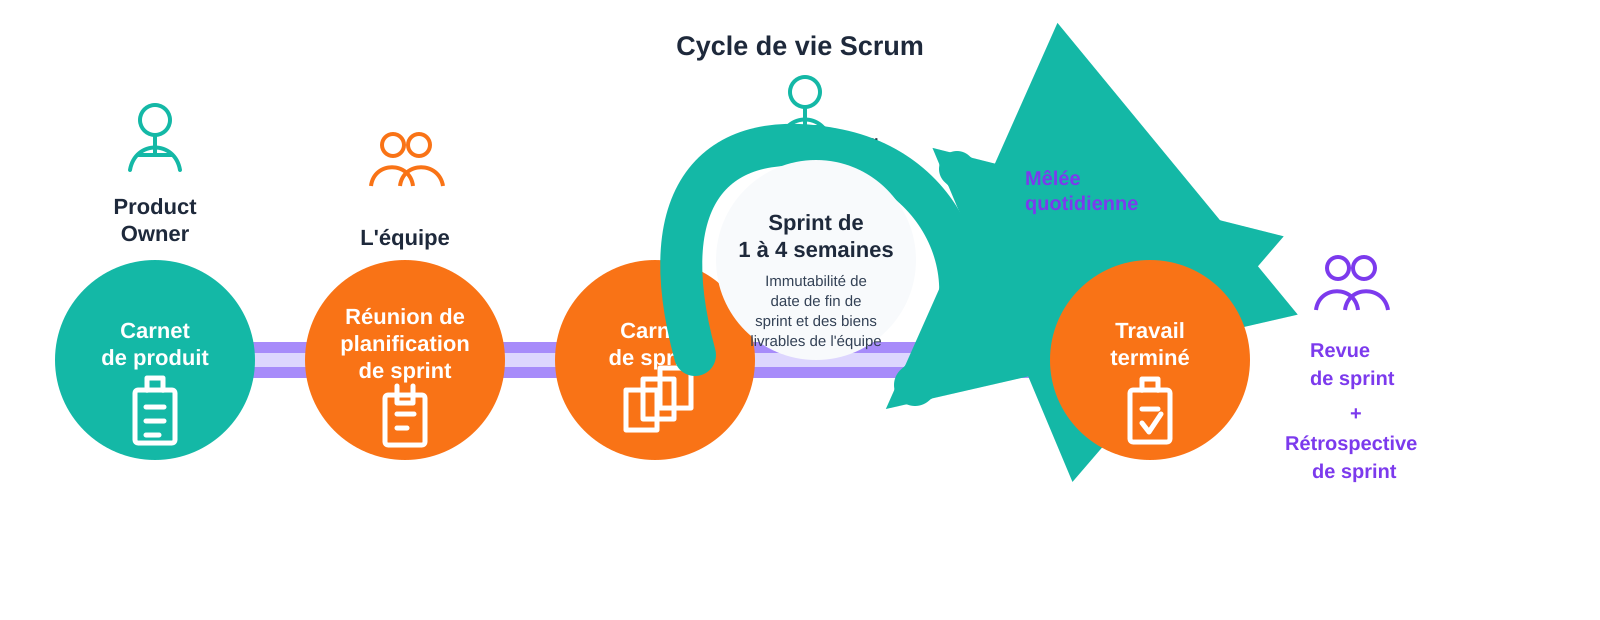
\includegraphics[width=0.70\textwidth]{img/scrum_cycle.png}}{\fbox{\parbox[c][3cm][c]{0.70\textwidth}{\centering Cycle de vie Scrum}}}
    \caption{Cycle de vie de la méthodologie Scrum}
    \label{fig:scrum-cycle}
\end{figure}

\section*{Conclusion}

Dans ce chapitre, nous avons présenté le contexte général du projet ainsi que l'organisme d'accueil, ASSURANCES MAGHREBIA. Nous avons ensuite exposé les enjeux liés au tri sélectif des déchets, analysé les limites des solutions existantes et présenté la solution proposée, \textit{EcoRewind}. Enfin, nous avons défini le formalisme UML et la méthodologie Scrum adoptés pour guider la conception et la réalisation de la plateforme. Le chapitre suivant sera consacré à l'analyse et à la spécification des besoins du système.
